\documentclass{amsart}
\usepackage{tikz}
\usetikzlibrary{arrows}
\begin{document}

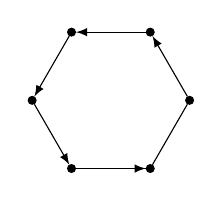
\begin{tikzpicture}
\tikzstyle{every node}=[draw,fill,shape=circle,inner sep=1pt];
\node (v1) at ( 0:1) {};
\node (v2) at ( 60:1) {};
\node (v3) at (2*60:1) {};
\node (v4) at (3*60:1) {};
\node (v5) at (4*60:1) {};
\node (v6) at (5*60:1) {};
\foreach \from/\to in {v1/v2, v2/v3, v3/v4, v4/v5, v5/v6}
    \draw [->,>=latex] (\from) -- (\to);
\foreach \from/\to in {v5/v6, v6/v1}
    \draw (\from) -- (\to);
\end{tikzpicture}
\end{document} 